\input{preamble.tex}
\newcommand{\C}{\mathcal{C}}
\usepackage{makecell} % commande \thead, dans l'exo 1

\begin{document}
\pagestyle{fancy}
\fancyhead[L]{Seconde}
\fancyhead[C]{\textbf{DS n°4 — évolution chiffrée}}
\fancyhead[R]{\today}

\reversemarginpar

\null\vspace{-30pt}
Nom / Prénom : \\

Consignes particulières : 
\begin{itemize}[label=$\bullet$]
	\item 
	La calculatrice est \textbf{autorisée}.
	\item 
	L'exercice \ref{exe:1} peut être fait entièrement sur la feuille d'évaluation. Écrire son nom avant de rendre le sujet pour qu'il soit corrigé.
	\item 
	Toute trace de recherche est prise en compte.
	%\item 
	%L'abbréviation $\tq$ signifie ``tel que''.
\end{itemize}

\hrule

\exe{4}{
	Vrai ou faux ? Cocher la case correspondante (aucune justification n'est attendue). \\
	\vspace{-20pt}
	\begin{center}
	\begin{tabular}{c c c}
		\hspace{10cm} & Vrai & Faux \\
		Si on multiplie une quantité par $\frac78$ elle augmente & \resizebox{10pt}{!}{$\square$} & \resizebox{10pt}{!}{$\square$}   \\
		Une variation relative est toujours positive & \resizebox{10pt}{!}{$\square$} & \resizebox{10pt}{!}{$\square$}   \\
		$90 \% < 1$ & \resizebox{10pt}{!}{$\square$} & \resizebox{10pt}{!}{$\square$}   \\
		\thead{Si une quantité exprimée en mètres évolue, \\
		sa variation absolue peut être exprimée en mètres} & \resizebox{10pt}{!}{$\square$} & \resizebox{10pt}{!}{$\square$}   \\
	\end{tabular}
	\end{center}
}{exe:1}{
Les réponses sont, dans l'ordre : Faux, faux, vrai, vrai.
}

\exe{4}{
Déterminer, pour chaque cas, le taux (en $\%$) d'évolution \textbf{totale} :
\begin{enumerate}[label=(\alph*)]
\item Une augmentation de $18 \%$ suivie d'une augmentation de $7 \%$.
\item Une baisse de $20 \%$ suivie d'une augmentation de $20 \%$.
\item Une augmentation d'une proportion 0,25 suivie d'une baisse d'une proportion 0,8.
\item Deux baisses successives de $50 \%$.
\end{enumerate}
}{exe:2}{
\begin{enumerate}[label=(\alph*)]
\item On calcule $1,18 \times 1,07 = 1,2626$, ce qui correspond à une augmentation de $26,26 \%$.
\item Une baisse de $4 \%$.
\item Une baisse de $75 \%$.
\item A nouveau, une baisse de $75 \%$.
\end{enumerate}
}

\exe{2}{
Déterminer, pour chaque cas, le taux (en $\%$) d'évolution \textbf{réciproque} :
\begin{enumerate}[label=(\alph*)]
\item Une augmentation de $23 \%$.
\item Une baisse de $4 \%$.
\end{enumerate}
}{exe:3}{
\begin{enumerate}[label=(\alph*)]
\item On calcule $\frac1{1,23} - 1$ soit une baisse d'environ $18,7 \%$.
\item Une augmentation d'environ $4,2 \%$.
\end{enumerate}
}

\exe{2}{
Dans une classe, $14 \%$ des élèves sont gauchers. Parmi les gauchers, $8 \%$ portent des chaussures rouges.
Estimer la proportion de v
}{exe:4}{
On note $C$ l'ensemble des élèves de la classe, $G$ l'ensemble des gauchers et $R$ l'ensemble des gauchers à chaussures rouges.
On a :
\[ p_G = 0,14 \quad \text{et} \quad p_{R/G} = 0,08 \]
On en déduit $p_R = 0,14 \times 0,08 = 0,0112$, soit $1,12 \%$ de gauchers à chaussures rouges dans la classe.
}

\exe{2}{
Dans chaque cas, déterminer la valeur manquante :
\begin{enumerate}[label=(\alph*)]
\item La valeur initiale d'une quantité dont la valeur finale est égale à $x_2 = 13$ et la variation relative égale à $\frac58$.
\item La valeur finale d'une quantité dont la valeur initiale est égale à $x_1=99$ et la variation absolue est égale à $-100$. 
\end{enumerate}
}{exe:4}{
\begin{enumerate}[label=(\alph*)]
\item On résout :
\[ \dfrac{13-x_1}{x_1} = \dfrac58 \iff 13 - x_1 = \dfrac58 x_1 \iff 13 = \dfrac{13}8 x_1 \iff x_1 = 8 . \]
\item On résout :
\[ x_2 - 99 = -100 \iff x_2 = -1 . \]
\end{enumerate}
}

\exe{2}{
Une colonie de 10 puces s'installe sur le dos d'un chat. Chaque jour, la taille de la colonie (le nombre de puces) augmente de $2 \%$.
Estimer la taille de la colonie après 1 an (365 jours) sans traitement anti-parasitaire.
}{exe:5}{
Après un jour, il y aura $10 \times (1,02)$ puces sur le dos du chat.
En utilisant la formule des évolutions successives, on en déduit qu'après 2 jours il y aura $10 \times (1,02)^2$ puces sur le dos du chat.
En itérant ce raisonnement, on en déduit qu'il y aura $10 \times (1,02)^365 \approx 13~774$ puces sur le dos du chat après un an.
Pauvre bête.
}

\exe{4}{
On considère la fonction suivante :
\[ \begin{array}{c c c c}
f : & \R & \to & \R \\
& x & \mapsto & \dfrac45 x
\end{array} \]
\begin{enumerate}
\item Esquisser la représentation graphique de $f$ dans le repère ci-dessous :
\begin{center}
	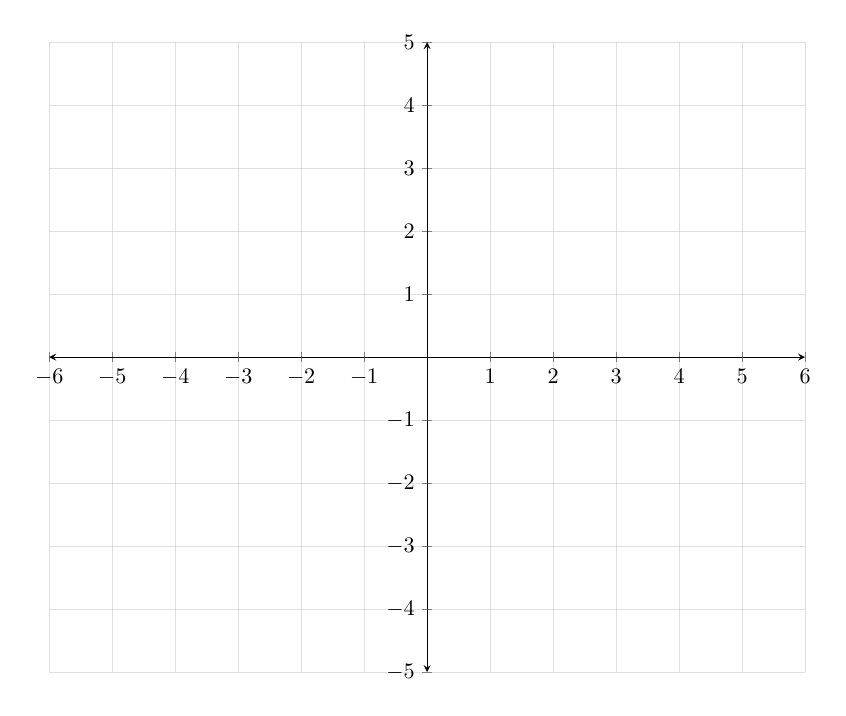
\begin{tikzpicture}[>=stealth, scale=.8]
		\begin{axis}[xmin = -6, xmax=6, ymin=-5, ymax=5, axis x line=middle, axis y line=middle, axis line style=<->, xlabel={}, ylabel={}, grid=both, grid style = {opacity=.5}, clip=false, xtick distance = 1, ytick distance=1, x=1cm, y=1cm]
		\end{axis}
	\end{tikzpicture}
\end{center}
\item Donner les éventuels antécédent de 80 par $f$.
\item Donner la variation relative entre $x$ et $f(x)$ pour $x$ un réel quelconque.
\item Existe-t-il $x$ tel que $f(x) > x$ ? Justifier.
\end{enumerate}
}{exe:6}{
\begin{enumerate}
\item Le tracé
\begin{center}
	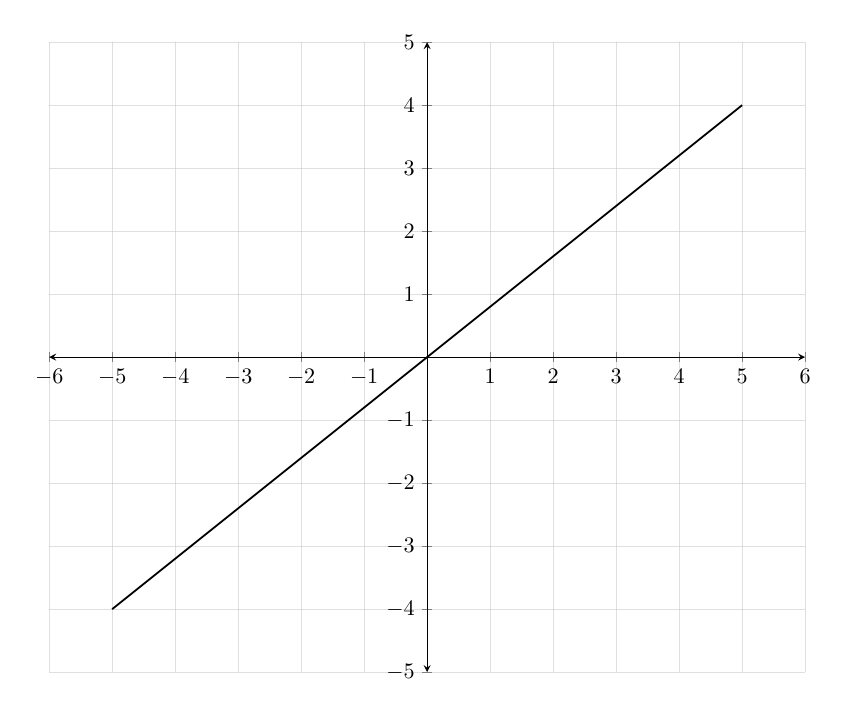
\begin{tikzpicture}[>=stealth, scale=.8]
		\begin{axis}[xmin = -6, xmax=6, ymin=-5, ymax=5, axis x line=middle, axis y line=middle, axis line style=<->, xlabel={}, ylabel={}, grid=both, grid style = {opacity=.5}, clip=false, xtick distance = 1, ytick distance=1, x=1cm, y=1cm]
		\addplot[thick,samples=400] (x,{4/5*x});
		\end{axis}
	\end{tikzpicture}
\end{center}
\item On résout $\frac45 x = 80$ soit $x=100$. L'antécédent est unique.
\item On calcule :
\[ \dfrac{f(x)-x}{x} = \dfrac{\frac45 x-x}{x} = -\dfrac15 \]
\item On résout :
\[ f(x) > x \iff \dfrac45 x > x \iff -\dfrac15 x > 0 \iff x < 0 \]
Il existe donc une infinité de $x$ vérifiant $f(x) > x$, ce sont les éléments de l'intervalle $]-\infty; 0[$.
\end{enumerate}
}

\exe{}{
(Bonus) \\
Soient $E_1, E_2, E_3$ des sous-populations emboîtées telles que :
\[ E_3 \subset E_2 \subset E_1 \subset E \]
On suppose que la sous-population $E_3$ représente respectivement $25 \%$ de la sous-population $E_2$, et $5 \%$ de la population $E$.
On suppose aussi que la sous-population $E_1$ représente $66 \%$ de la population $E$. \newline
Estimer la proportion représentée par la sous-population $E_2$ dans la sous-population $E_1$.
}{exe:b}{
On a $p_{E_3/E_2} = 25 \%, p_{E_3} = 5 \%$ et $p_{E_1} = 66 \%$, or :
\begin{align*}
p_{E_3} & = p_{E_3 / E_2} \times p_{E_2} \\
p_{E_3} & = p_{E_3 / E_2} \times p_{E_2 / E_1} \times p_{E_1} 
\end{align*}
en appliquant deux fois la formule pour les populations imbriquées. On résout ensuite :
\[ 0,05 = 0,25 \times p_{E_2 / E_1} \times 0,66 \iff p_{E_2 / E_1} = \dfrac{0,25}{0,66 \times 0,05} \approx 0,30 . \]
La la sous-population $E_2$ représente environ $30 \%$ de la sous-population $E_1$.
}

%\exe{}{
%(Exercice bonus) \\
%Soient $E_1, E_2, \dots, E_{100}$ des sous-populations emboîtées telles que :
%\[ E_{100} \subset E_{99} \subset \cdots \subset E_2 \subset E_1 . \]
%On suppose que la proportion d'éléments de $E_{i}$ appartenant à $E_{i+1}$ est consante égale à $p$ pour tout $i$ de 1 à 100.
%Estimer la valeur de $p$ pour que la proportion d'éléments de $E_1$ appartenant à $E_{100}$ soit supérieure à $0,36$.
%}{exe:b}{
%
%}


%%%%%%%%%%%%

\newpage
\fancyhead[C]{\textbf{Solutions}}
\shipoutAnswer

\end{document}
 